\chapter{Specyfikacja wewnętrzna}
\label{ch:05}

\section{Architektura systemu}

\note{W tej części pracy należy opisać, jakie komponenty składają się na system. Należy zaznaczyć, jakie są relacje między nimi. Można również opisać, jakie wzorce projektowe zostały zastosowane. Głównie chodzi o to, aby czytelnik mógł zrozumieć, jak działa system.}

Kompletny system składa się z czterech głównych komponentów, które komunikują się ze sobą w celu zapewnienia pełnej funkcjonalności. Poniżej zostały przedstawione opisy każdego z nich.

\subsection{Frontend}

Głównym interfejsem użytkownika jest aplikacja webowa stworzona przy użyciu frameworka \texttt{Vue.js}. Zapewnia użytkownikowi dostęp do większości funkcji systemu, a w zależności od roli użytkownika, pozwala na wykonanie innych czynności. Aplikacja została zaprojektowana w taki sposób, aby była przejrzysta i intuicyjna w obsłudze. Dzięki temu, użytkownik może szybko i sprawnie wykonywać swoje codzienne obowiązki. Odrębne od siebie panele zostały umieszczone w kartach pojawiających się na widoku, dzięki czemu użytkownik wie dokładnie w którym miejscu aplikacji się znajduje i jakie ma możliwości.

\subsection{Backend}

Serwer aplikacyjny został stworzony przy użyciu frameworka \texttt{Spring Boot}. Zapewnia on komunikację między bazą danych, a pozostałymi komponentami systemu. Jest odpowiedzialny za przetwarzanie żądań klienckich oraz zwracanie odpowiedzi w postaci danych, w formacie \texttt{JSON}. Serwer aplikacyjny jest również odpowiedzialny za autoryzację i autentykację użytkowników oraz zarządzanie sesjami. Użytkownicy nie mają bezpośredniego dostępu do serwera.

\subsection{Aplikacja mobilna}

Głównym zadaniem aplikacji mobilnej jest możliwość dodawania kart dostępowych dla poszczególnych użytkowników. Odbywa się to poprzez przyłożenie tagu NFC (ang. \english{Near Field Communication}) do telefonu z zainstalowaną aplikacją, a następnie przypisanie go do konkretnego użytkownika. Szczegółowy opis tego procesu został opisany w rozdziale \ref{sec:addNfc}.

\subsection{Układ mikroprocesorowy}

Układ mikroprocesorowy jest odpowiedzialny za odczytywanie tagów NFC oraz przesyłanie informacji do serwera aplikacyjnego. Następnie serwer zwraca informację o przyznaniu dostępu do systemu. Układ mikroprocesorowy jest zasilany z wbudowanego portu Micro USB, co umożliwia bardzo proste podłączenie go do źródła zasilania. Dokumentacja techniczna mikrokontrolera \cite{bib:picoWdatasheet} precyzuje również podłączenie innego źródła zasilania bez użycia wbudowanego portu.

\section{Struktura bazy danych}

\note{W tej części pracy należy opisać, jakie tabele i relacje między nimi występują w bazie danych. Można dodać diagramy ERD.}

Baza danych obsługująca system składa się z kilkunastu tabel, które przechowują informacje o wszelkich danych w systemie. Na rysunku \ref{fig:dbDiagram} został przedstawiony jej uproszczony schemat, a w kolejnych podrozdziałach zostaną opisane najważniejsze tabele oraz ich relacje.

\begin{figure}[H]
    \centering
    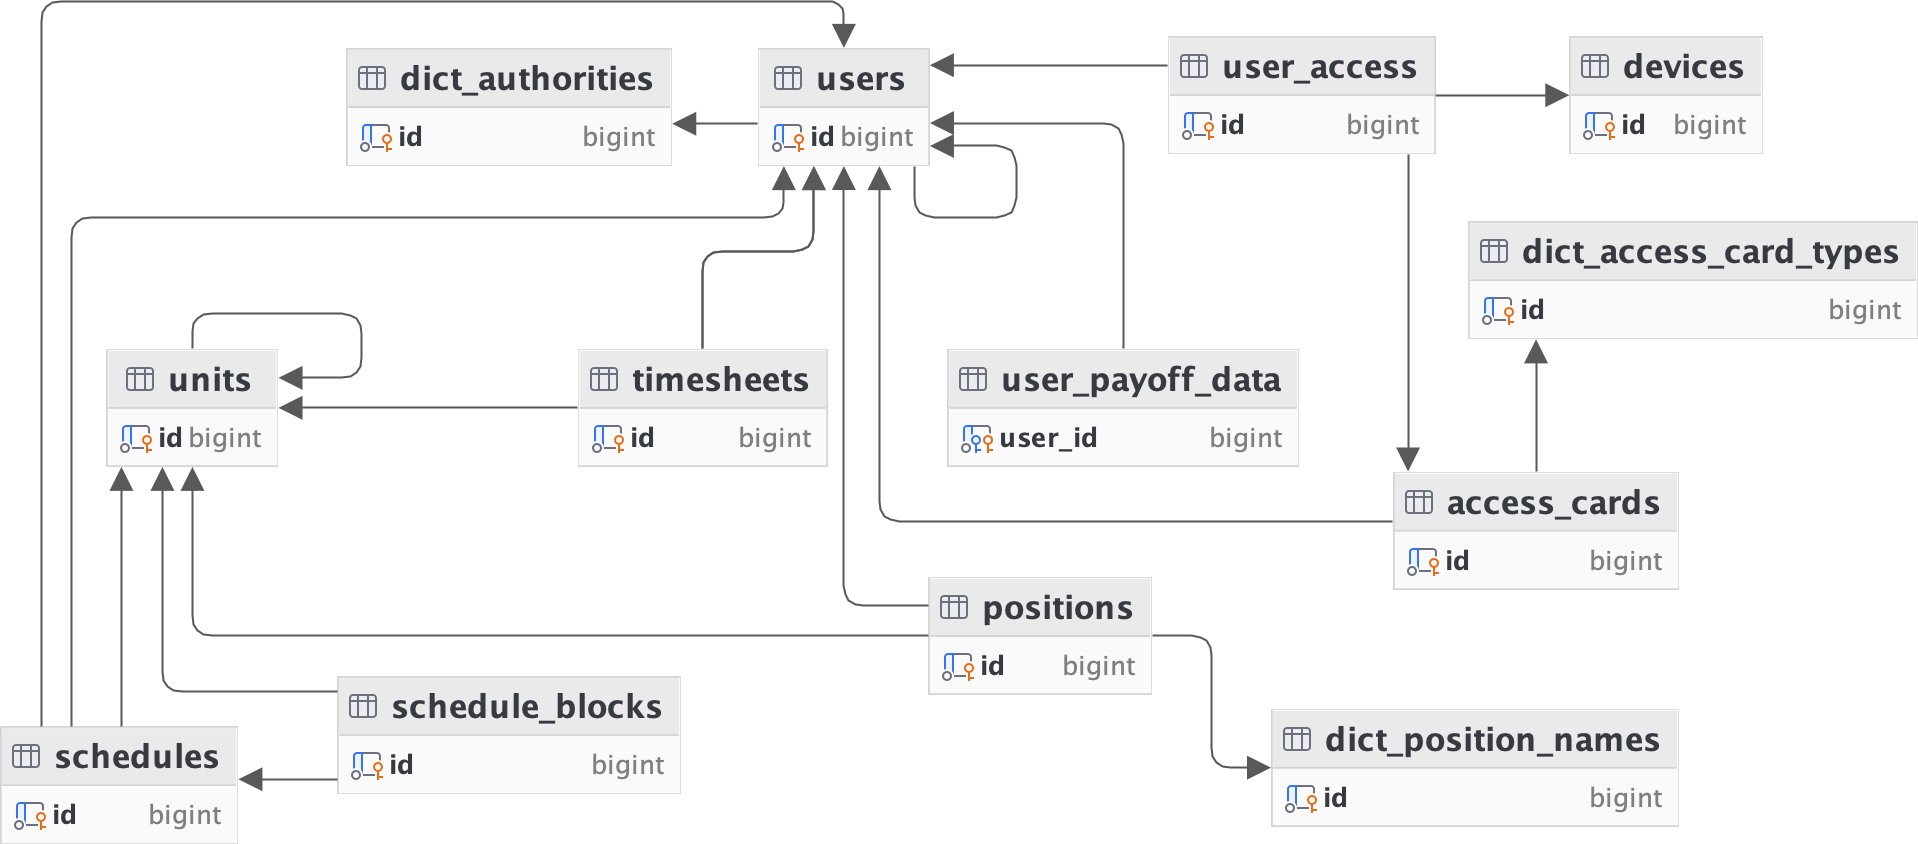
\includegraphics[width=\textwidth]{graf/dbDiagram.png}
    \caption{Uproszczony schemat bazy danych}
    \label{fig:dbDiagram}
\end{figure}

\subsection{Tabele użytkowników}

\begin{figure}[H]
    \centering
    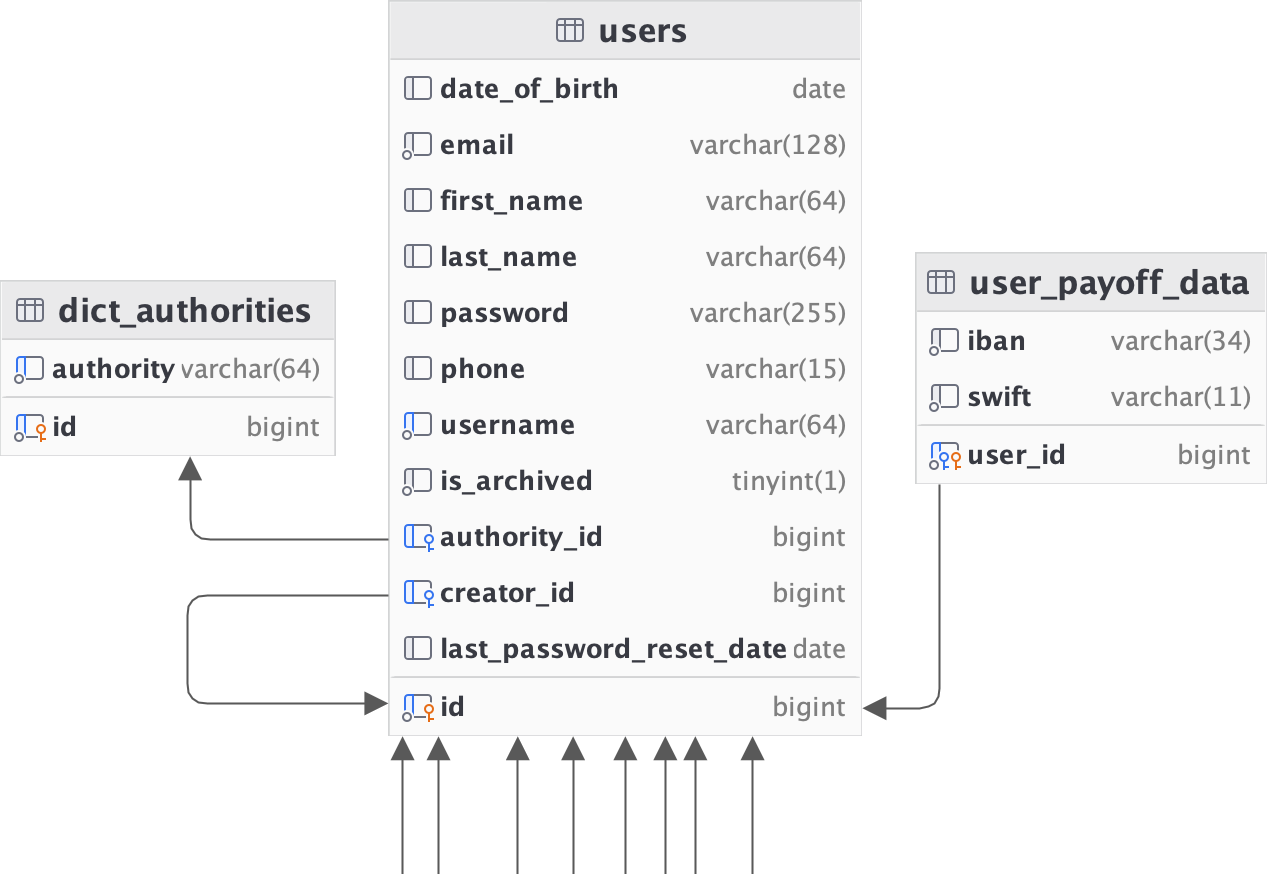
\includegraphics[width=0.7\textwidth]{graf/usersTable.png}
    \caption{Schemat tabel użytkowników}
    \label{fig:usersTable}
\end{figure}

Główną tabelą przechowującą informacje o użytkownikach jest tabela \texttt{USERS}. Zawiera ona dane personalne, takie jak imię, nazwisko, adres e-mail i numer telefonu. Dodatkowo do tabeli wpisane są dane do logowania: nazwa użytkownika i hasło; oraz informacja o użytkowniku, który  utworzył dany wpis. Każdy użytkownik ma przypisaną jedną z ról z tabeli \texttt{DICT\_AUTHORITIES}, która określa jego uprawnienia w systemie - w relacji wiele do jednego. Relacją jeden do jednego jest połączona tabela \texttt{USER\_PAYOFF\_DATA} zawierające dane o koncie bankowym użytkownika. W tabeli \texttt{USERS} znajduje się również pole \texttt{is\_archived}, które określa, czy użytkownik jest aktywny w systemie.

\subsection{Tabele jednostek organizacyjnych}

\begin{figure}[H]
    \centering
    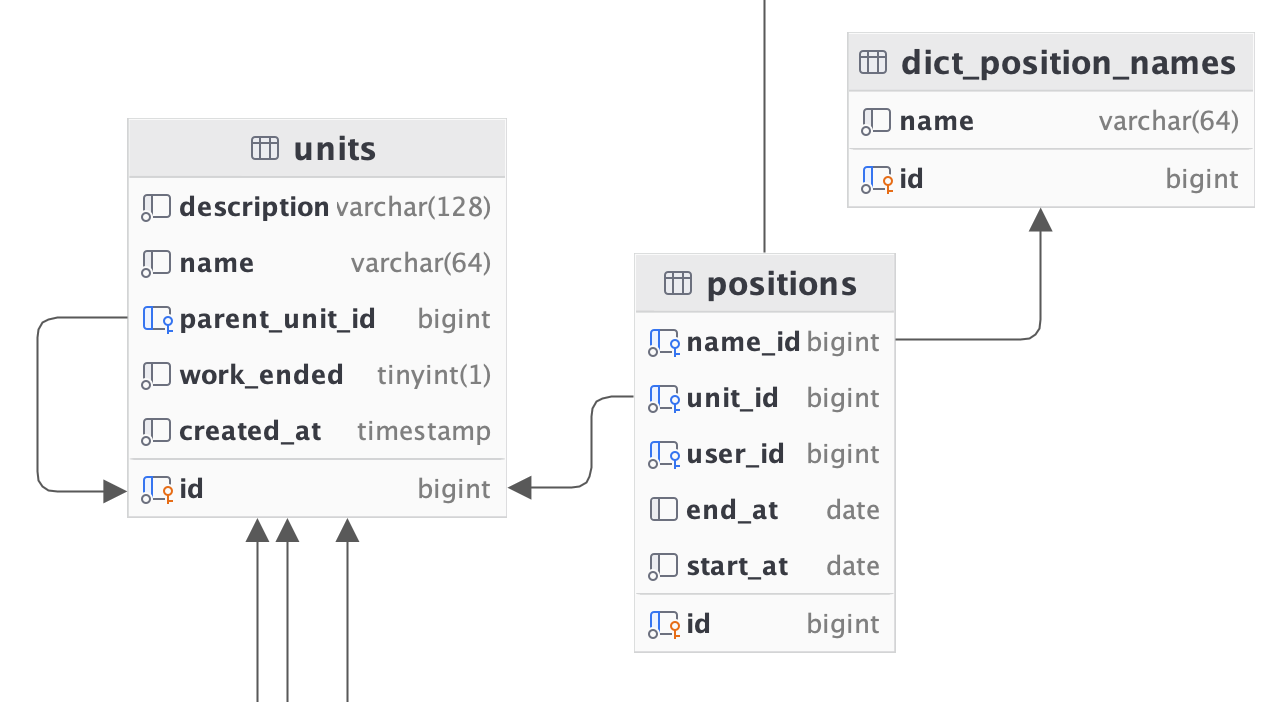
\includegraphics[width=0.8\textwidth]{graf/unitsTable.png}
    \caption{Schemat tabel jednostek organizacyjnych}
    \label{fig:organizationalUnitsTable}
\end{figure}

Wszystkie jednostki organizacyjne są przechowywane w tabeli \texttt{UNITS} zawierającej dane o nazwie jednostki, jej opisie, jednostce nadrzędnej oraz dacie utworzenia. Pole \texttt{work\_ended} określa, czy jednostka jest aktywna. Użytkownicy są przypisani do jednostki organizacyjnej poprzez tabelę \texttt{positions} będącą tabelą łącznikową między tabelami \texttt{USERS} i \texttt{UNITS}. Znajdują się w niej dane o dacie rozpoczęcia pracy na danym stanowisku oraz dacie zakończenia pracy, a także odwołanie do tabeli słownikowej, zawierającej nazwy stanowisk. Tabela \texttt{POSITIONS} jest szczególnie ważna przy odczytywaniu harmonogramów pracy.

\subsection{Tabele harmonogramów}

\begin{figure}[H]
    \centering
    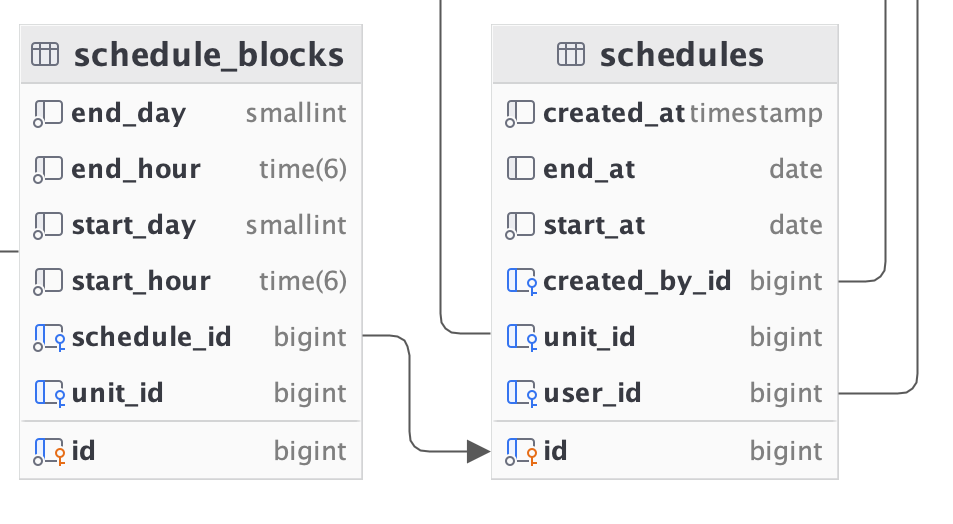
\includegraphics[width=0.7\textwidth]{graf/scheduleTable.png}
    \caption{Schemat tabel harmonogramów}
    \label{fig:schedulesTable}
\end{figure}

Na każdy z harmonogramów składa się pojedynczy rekord w tabeli \texttt{SCHEDULES} oraz pewna liczba rekordów w tabeli \texttt{SCHEDULE\_BLOCKS}. Pierwsza z nich zawiera informacje o dacie rozpoczęcia i zakończenia harmonogramu, jego utworzenia oraz odwołanie do jednostki organizacyjnej lub użytkownika, którego dotyczy. Tabela \texttt{SCHEDULE\_BLOCKS} odpowiada za przechowywanie pojedynczych bloków czasowych w harmonogramie opisując ich dzień i godzinę rozpoczęcia oraz zakończenia oraz jednostkę, której dotyczą. Tabele są powiazane relacją jeden do wielu - jeden harmonogram może zawierać wiele bloków czasowych.

\subsection{Tabele kart dostępowych}

\begin{figure}[H]
    \centering
    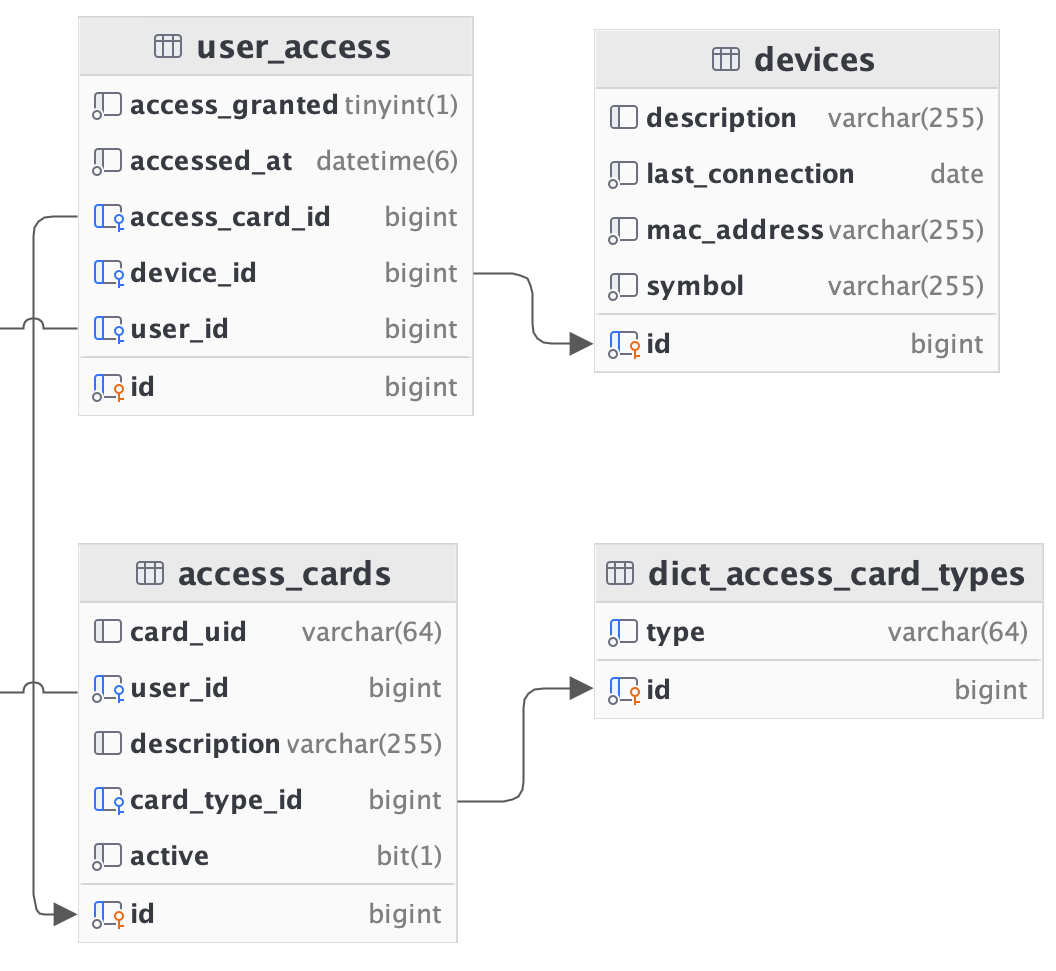
\includegraphics[width=0.7\textwidth]{graf/acTable.png}
    \caption{Schemat tabel kart dostępowych}
    \label{fig:accessCardsTable}
\end{figure}

Karty dostępowe użytkowników są przechowywane w tabeli \texttt{ACCESS\_CARDS} zawierającej informacje o numerze seryjnym, jej właścicielu opisie, typie karty oraz statusie. Dzięki ostatniej z właściwości możliwe jest przypisanie dwóm użytkownikom jednej karty w różnych okresach czasu. Każda autoryzacja użytkownika jest zapisywana w tabeli \texttt{USER\_ACCESS} wpisując do niej datę i godzinę, id użytkownika, id czytnika, id karty dostępowej oraz status autoryzacji. Umożliwia to późniejsze analizowanie historii autoryzacji.

Tabela \texttt{DEVICES} przechowuje informacje o czytnikach kart - ich opis, datę ostatniego uruchomienia, adres MAC (ang. \english{Media Access Control address}) oraz symbol, którym identyfikuje się w systemie.

\subsection{Tabele słownikowe}

W bazie danych znajdują się trzy tabele słownikowe zawierające dane, które nie zmieniają się w czasie działania systemu. Każda z nich poprzedzona jest prefiksem \texttt{DICT\_}. Są to:

\begin{itemize}
    \item \texttt{DICT\_AUTHORITIES} zawierająca role użytkowników, równoznaczne z uprawnieniami,
    \item \texttt{DICT\_ACCESS\_CARD\_TYPES} zawierająca typy kart dostępowych dla łatwiejszego rozróżnienia tagów NFC,
    \item \texttt{DICT\_POSITION\_NAMES} zawierająca nazwy stanowisk przypisanych pracownikom.
\end{itemize}

Do tabel \texttt{DICT\_ACCESS\_CARD\_TYPES} i \texttt{DICT\_POSITION\_NAMES} mogą zostać dodane nowe rekordy, lecz nie jest możliwe ich usunięcie. Takie ograniczenie zapewnia integralność danych w systemie i zapobiega błędom w działaniu aplikacji.

Dane mogą dodawać jedynie administratorzy systemu.

\section{Modele i struktury danych}

\note{W tej części pracy należy opisać, jakie modele danych zostały zastosowane w systemie. Należy zaznaczyć, jakie są relacje między nimi.}

\subsection{Model użytkownika}

\section{Algorytmy}

\subsection{Rejestracja}

\subsection{Logowanie}

\begin{figure}[H]
    \centering
    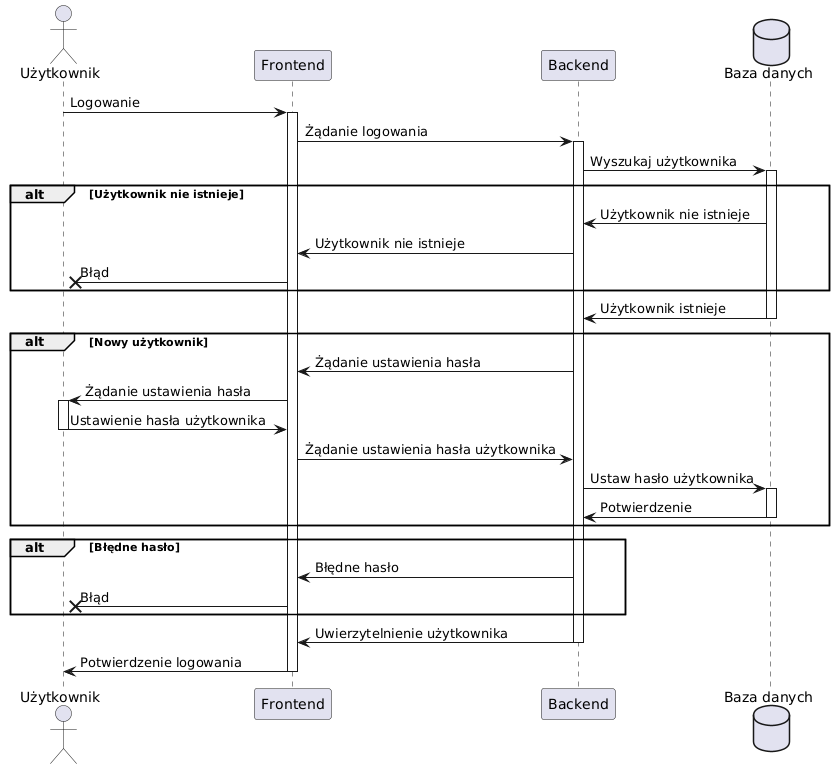
\includegraphics[width=0.8\textwidth]{graf/loginSequence.png}
    \caption{Diagram czynności logowania}
    \label{fig:login}
\end{figure}
% //www.pantum.com/plantuml/png/VP8nRiCm34LtdKB8dWju288CdOgYIz2PigX6iIC5jbJN7WFq43rBEzRtAeceK6pKcJpyh__9Hs_R04s8frf06NmZz-Dt7ohVELj9QAMBuaowBUqPN90FZNS1dMR9u4JQGLabHQ7G4411YtArWm6a1jUNXnMBMWaXN9Jh3IN8GZxwLz-1iyW3s3S8oCa6rnl5ylZryw5PbdKoGZPIaK9EqegiBtqxn0gECkOTifcBeGwJ1JdMje4-HnfPSHANBdfIcxdhCUnv9t9aseqN6byG5uhdZMOFSpdEvtpoNN-xYL24n4oHH3fUPv6Oo0EqumK4StFnhYaZuUkwoAd5_i-4oJI5gF7cJJfEiLmnUysJQqMRi-tgy8j7Ig0A-Um3PJPweDmv80RAa9ZlftQOGZEZkM3mdvja-vwRXZvWxQuGbhPNwRuSDHin_w2t3moABLN5K_qB

\subsection{Harmonogramowanie}

\subsection{Przypisanie nowej karty dostępowej}

\section{Użyte biblioteki i frameworki}

\note{Ta część może się znaleźć przy przeglądzie technologii.}